\documentclass[polish,aspectratio=169]{beamer}

% wide screen
% \documentclass[aspectratio=169]{beamer}


%%% YOUR PACKAGES HERE %%%
\usepackage{comment}
\usepackage{hyperref}
\usepackage[backend=biber, style=numeric, bibstyle=ieee,
            sorting=none, isbn=false, urldate=ymd,
            doi=false, url=true]{biblatex}
\addbibresource{bibliography/bibliography.bib}
\renewbibmacro{in:}{}
\usepackage{subfigure}
\usepackage{graphicx}
\usepackage{geometry}
\usepackage{float}
\usepackage{listings}
\usepackage{xcolor}

\newcommand{\refrys}[1]{Rys.~\ref{#1}}
\newcommand{\reflist}[1]{List.~\ref{#1}}
\newcommand{\refEq}[1]{Równ.~\ref{#1}}
% \usepackage{tikz} 
% \usetikzlibrary{graphs,graphs.standard,automata}


\definecolor{keywordcolor}{rgb}{0.1,0.1,0.8}
\definecolor{stringcolor}{rgb}{0.7,0.1,0.1}
\definecolor{commentcolor}{rgb}{0.3,0.7,0.3}
\definecolor{backgroundcolor}{rgb}{0.95,0.95,0.95}
\lstdefinelanguage{FSharp}{
    keywords={let, match, with, in, function, if, then, else, rec, type, module, open},
    keywordstyle=\color{keywordcolor}\bfseries,
    sensitive=true,
    comment=[l][\color{commentcolor}\itshape]{//},
    morecomment=[s][\color{commentcolor}\itshape]{(*}{*)},
    string=[b]",
    stringstyle=\color{stringcolor},
    basicstyle=\ttfamily,
    numbers=left,
    numberstyle=\tiny\color{gray},
    backgroundcolor=\color{backgroundcolor},
    showstringspaces=false
}
% polish language
\usepackage[polish]{babel}
\usepackage{polski}



%%% IMPORT PG PRESENTATION STYLE %%%
% THIS IS GDANSK UNIVERSITY OF TECHNLOGOGY (PG) PRESENTATION TEMPLATE
% Creator: Jan Cychnerski <jan.cychnerski@eti.pg.edu.pl>
% Copyleft 2019


% PG THEME OPTIONS

\usetheme{Boadilla}
\usecolortheme{default}
\usefonttheme{professionalfonts}

% colors

\definecolor{PGBlue}{RGB}{0,56,101}
\definecolor{PGRed}{RGB}{193,10,39}
\definecolor{PGSilver}{RGB}{200,200,200}
\definecolor{PGBlack}{RGB}{0,0,0}

% PGBlue
\setbeamercolor{frametitle}{fg=PGBlue}
\setbeamercolor{normal text}{fg=PGBlue}
\setbeamercolor{structure}{fg=PGBlue}
\setbeamercolor{item}{fg=PGBlue}

% PGRed
\setbeamercolor{alerted text}{fg=PGRed}
\setbeamercolor{item projected}{fg=PGRed}

% white
\setbeamercolor{title}{fg=white}
\setbeamercolor{titlelike}{fg=white}
\setbeamercolor{subtitle}{fg=white}

% enumerate and itemize styles

\setbeamertemplate{itemize item}{\bfseries\color{PGRed}\raise1pt\hbox{\donotcoloroutermaths$\bullet$}}
\setbeamertemplate{itemize subitem}{\color{PGRed}\raise0.5pt\hbox{--}}
\setbeamertemplate{itemize subsubitem}{\color{PGRed}\tiny\raise1.5pt\hbox{\donotcoloroutermaths$\bullet$}}

\setbeamertemplate{enumerate item}{\bfseries\color{PGRed}\insertenumlabel.}
\setbeamertemplate{enumerate subitem}{\color{PGRed}\insertsubenumlabel.}
\setbeamertemplate{enumerate subsubitem}{\color{PGRed}\insertsubsubenumlabel.}
\setbeamertemplate{enumerate mini template}{\insertenumlabel}


% disable navigation

\beamertemplatenavigationsymbolsempty

% additional commands

\newcommand*{\vcenteredhbox}[1]{\begingroup
\setbox0=\hbox{#1}\parbox{\wd0}{\box0}\endgroup}

\graphicspath{{pgbeamer/}}


\usepackage{iflang}
\IfLanguageName{polish}{
\newcommand{\pglogobig}{pg-logo-big-pl}
\newcommand{\pglogosmall}{pg-logo-small-pl}
}{
\newcommand{\pglogobig}{pg-logo-big-en}
\newcommand{\pglogosmall}{pg-logo-small-en}
}


% FRAME TITLE LOGO
\addtobeamertemplate{frametitle}{\vcenteredhbox{\includegraphics[height=8mm]{\pglogosmall}}\bfseries}{}


\newcommand{\pgtitleframe}{{
% PG TITLE PAGE

\setbeamercolor{background canvas}{bg=PGBlue}
\setbeamercolor{title}{fg=white}
\setbeamercolor*{date}{fg=white}
\setbeamercolor*{author}{fg=white}

\setbeamertemplate{footline}{}

\begin{frame}[noframenumbering]
\centering
\vspace{1cm}
\includegraphics[height=3cm]{\pglogobig}
\vspace{5mm}
\maketitle
\end{frame}
}}

\newcommand{\pglastframe}{{
% PG LAST PAGE

\setbeamercolor{background canvas}{bg=PGBlue}
\setbeamercolor{title}{fg=white}
\setbeamercolor*{date}{fg=white}
\setbeamercolor*{author}{fg=white}

\setbeamertemplate{footline}{}

\begin{frame}[noframenumbering]
\centering
\vspace{1cm}
\includegraphics[height=5cm]{\pglogobig}
\end{frame}
}}



%%% YOUR OPTIONS HERE %%%

\title[Czy na MuZero można odpalić Doom'a?]{Czy na MuZero można odpalić Doom'a?}
% \subtitle{Jak testować zachowanie, a nie przypadki}
\author{Paulina Brzęcka \and Marek Borzyszkowski}
\date{\today}

\setbeamercovered{invisible}
\begin{document}

\pgtitleframe


\begin{frame}{Jak działa MuZero}
  Istnieje wiele koncepcji testowania oprogramowania, jedną z nich jest testowanie na podstawie właściwości \cite{pbt_bib}.
  \onslide<2->{Dziś dowiecie się:
      \begin{enumerate}
      \item na czym polega testowanie na podstawie właściwości.
      \item Czym różni się ono od klasycznego podejścia do testowania.
      \item Jakie są strategie testowania na podstawie właściwości. 
      \item Jak przy wykorzystaniu konceptu QuickCheck znaleźć wartości początkowe nieprzechodzące testy.
      \end{enumerate}
  }
\end{frame}
\section{Informacje na temat eksperymentu}
  \subsection{Literatura}
    Do zrozumienia problemu wykorzystano następujące pozycje:
    \begin{enumerate}
      \item \url{https://arxiv.org/pdf/1911.08265}
      \item \url{https://www.youtube.com/watch?v=c8SLNEpFSrs}
    \end{enumerate}

  \subsection{Przydatne repozytoria}
    Przykładowe implementacje MuZero:
    \begin{enumerate}
      \item \url{https://github.com/johan-gras/MuZero}
      \item \url{https://github.com/opendilab/LightZero}
      \item \url{https://github.com/werner-duvaud/muzero-general}
    \end{enumerate}
    Środowiska:
    \begin{enumerate}
      \item \url{https://github.com/Farama-Foundation/Arcade-Learning-Environment}
      \item \url{https://paperswithcode.com/dataset/dqn-replay-dataset}
      \item \url{https://github.com/clvrai/awesome-rl-envs}
      \item \url{https://github.com/Farama-Foundation/ViZDoom}
    \end{enumerate}
   
  \subsection{Framework}
    Do powtórzenia eksperymentu będziemy korzystać z 
    \begin{enumerate}
      \item pytorch
      \item opencv
      \item numpy
      \item ray
    \end{enumerate}

  \subsection{Co będzie przedmiotem eksperymentu}
    Przeprowadzenie testów na 
    \begin{enumerate}
      \item test na prostych środowiskach,
      \item test na atari,
      \item test na doom'ie.
    \end{enumerate}

  \subsection{Metryki i baseline}
    
      
        Wyuczenie agentów do poziomu przeciętnego człowieka, który grał parę godzin w grę.  
     
        \begin{tabular}[H]{||c c||} 
        \hline
        Game & Human \\ [0.5ex] 
        \hline\hline
        Atlantis & $29028.13$ \\ 
        \hline
        Bowling & $160.73$  \\
        \hline
        Breakout & $30.47$ \\
        \hline
        Crazy climber & $35829.41$  \\
        \hline
        Pacman & $6951.60$  \\
        \hline
        Pong & $14.59$  \\ [1ex] 
        \hline
        \end{tabular}

  \subsection{Sprzęt użyty w testach}
    Do testów wykorzystano 2 rodzaje komputerów:
    \begin{enumerate}
      \item Intel i7 13700k + 32GB ram + Nvidia RTX 4070 Ti,
      \item Intel i5 4590 + 32GB ram.
    \end{enumerate}  

\begin{frame}{Strategie}
    Testowanie na podstawie właściwości nie jest proste w zastosowaniu, przynajmniej przy pierwszej próbie.
    Istnieją jednak pewne schematy wskazujące drogę, jak stworzyć takie testy.
    \begin{enumerate}[<+->]
        \item Różne ścieżki, ten sam wynik
        \item Tam i z powrotem
        \item Są rzeczy niezmienne
        \item Z czasem rzeczy przestają się zmieniać
        \item Dziel i rządź
        \item Łatwiej zweryfikować niż zaimplementować
        \item Testowanie z wyrocznią
    \end{enumerate}
\end{frame}

\begin{frame}{Strategie - Różne ścieżki, ten sam wynik}
    \begin{columns}[t]
        \column{.5\textwidth}
            Jedną z podstawowych strategii skorzystanie z komutatywności niektórych operacji. Można to zrobić poprzez wykonanie operacji w różnej kolejności.\\
            \onslide<2->{
                Przykładem takiej strategii może być komutatywność dodawania, gdzie wykorzystano \texttt{add x y}, jak i odwrotność tej operacji \texttt{add y x}.\\ 
            }
            \onslide<3->{
                Innym przykładem jest test metody \texttt{sort} danej listy. 
                Wykonanie sortowania, a następnie dodanie do każdego elementu listy \texttt{1} powinno dać taki sam efekt jak dodanie \texttt{1} do każdego z elementów listy, a następnie jej posortowanie.
            }
        \column{.5\textwidth}
        \centering
        \begin{figure}
            \centering
            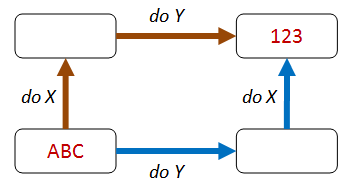
\includegraphics[width=1\textwidth]{images/property_commutative.png}
            \caption{Strategia - komutatywność}
            \label{fig:commutative_strategy}
        \end{figure}    
    \end{columns}
\end{frame}

\begin{frame}{Strategie - Różne ścieżki, ten sam wynik}
    \begin{columns}[t]
        \column{.5\textwidth}
            Jedną z podstawowych strategii skorzystanie z komutatywności niektórych operacji. Można to zrobić poprzez wykonanie operacji w różnej kolejności.\\
            Przykładem takiej strategii może być komutatywność dodawania, gdzie wykorzystano \texttt{add x y}, jak i odwrotność tej operacji \texttt{add y x}.\\ 
            Innym przykładem jest test metody \texttt{sort} danej listy. 
            Wykonanie sortowania, a następnie dodanie do każdego elementu listy \texttt{1} powinno dać taki sam efekt jak dodanie \texttt{1} do każdego z elementów listy, a następnie jej posortowanie.
        \column{.5\textwidth}
        \centering
        \begin{figure}
            \centering
            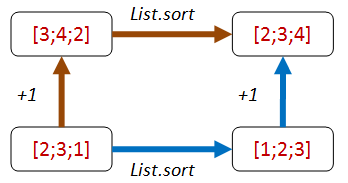
\includegraphics[width=1\textwidth]{images/property_list_sort1.png}
            \caption{Strategia - komutatywność}
            \label{fig:commutative_strategy_example}
        \end{figure}    
    \end{columns}
\end{frame}

\begin{frame}[fragile]{Strategie - Różne ścieżki, ten sam wynik}
    \begin{lstlisting}[language=FSharp, xleftmargin=-10pt,xrightmargin=-10pt,numbers=none, basicstyle=\ttfamily\small]
    let addThenSort_eq_sortThenAdd sortFn aList =
        let add1 x = x + 1
        
        let result1 = aList |> sortFn |> List.map add1
        let result2 = aList |> List.map add1 |> sortFn
        result1 = result2
    \end{lstlisting}
\end{frame}

\begin{frame}{Strategie - Różne ścieżki, ten sam wynik}    
    \begin{figure}
        \centering
        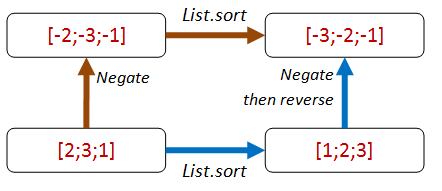
\includegraphics[width=0.5\textwidth]{images/property_list_sort3.png}
        \caption{Strategia - komutatywność}
        \label{fig:commutative_strategy_example_2}
    \end{figure}    
\end{frame}

\begin{frame}{Strategie - Tam i z powrotem}
    \begin{columns}[t]
        \column{.5\textwidth}
            Przykładem takiego testu mogą być przeciwne operacje matematyczne jak:
            \begin{itemize}[<+->]
                \item \texttt{dodawanie/odejmowanie}
                \item \texttt{mnożenie/dzielenie}
                \item \texttt{potęga/logarytm}.
            \end{itemize} 
            \onslide<4->{Innymi przykładami są operacje niekoniecznie matematyczne:}
            \begin{itemize}[<+->]
                \item \texttt{serializacja/deserializacja}
                \item \texttt{zapis/odczyt z pliku}
                \item \texttt{wstaw/sprawdź czy zawiera}.
                \item \texttt{odwrócenie listy/odwrócenie listy}
            \end{itemize} 
        \column{.5\textwidth}
        \centering
        \begin{figure}
            \centering
            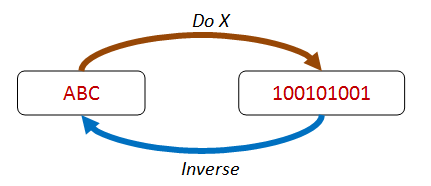
\includegraphics[width=1\textwidth]{images/property_inverse.png}
            \caption{Strategia - inwersja}
            \label{fig:inverse_strategy}
        \end{figure}    
    \end{columns}
\end{frame}

\begin{frame}{Strategie - Tam i z powrotem}
    \begin{columns}[t]
        \column{.5\textwidth}
            Przykładem takiego testu mogą być przeciwne operacje matematyczne jak:
            \begin{itemize}
                \item \texttt{dodawanie/odejmowanie}
                \item \texttt{mnożenie/dzielenie}
                \item \texttt{potęga/logarytm}.
            \end{itemize} 
            Innymi przykładami są operacje niekoniecznie matematyczne:
            \begin{itemize}
                \item \texttt{serializacja/deserializacja}
                \item \texttt{zapis/odczyt z pliku}
                \item \texttt{wstaw/sprawdź czy zawiera}.
                \item \texttt{odwrócenie listy/odwrócenie listy}
            \end{itemize} 
        \column{.5\textwidth}
        \centering
        \begin{figure}
            \centering
            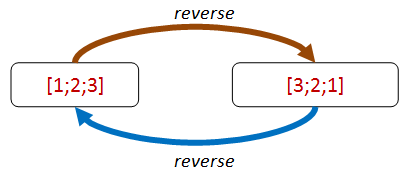
\includegraphics[width=1\textwidth]{images/property_list_rev_inverse.png}
            \caption{Strategia - inwersja}
            \label{fig:inverse_strategy_example}
        \end{figure}    
    \end{columns}
\end{frame}

\begin{frame}{Strategie - Są rzeczy niezmienne}
    \begin{columns}[t]
        \column{.5\textwidth}
            Czasami testowana funkcja przetwarzając dane zachowuje część ich właściwości.
            Chociażby funkcje \texttt{sort} lub \texttt{map} wykonane na liście \texttt{n} elementów, zwracaja odpowiednio zmodyfikowaną listę \texttt{n} elementową.
        \column{.5\textwidth}
        \centering
        \begin{figure}
            \centering
            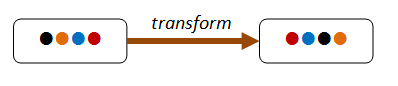
\includegraphics[width=1\textwidth]{images/property_invariant.png}
            \caption{Strategia - niezmienność}
            \label{fig:invariant_strategy}
        \end{figure}    
    \end{columns}
\end{frame}

\begin{frame}{Strategie - Są rzeczy niezmienne}
    \begin{columns}[t]
        \column{.5\textwidth}
            Czasami testowana funkcja przetwarzając dane zachowuje część ich właściwości.
            Chociażby funkcje \texttt{sort} lub \texttt{map} wykonane na liście \texttt{n} elementów, zwracaja odpowiednio zmodyfikowaną listę \texttt{n} elementową.
        \column{.5\textwidth}
        \centering
        \begin{figure}
            \centering
            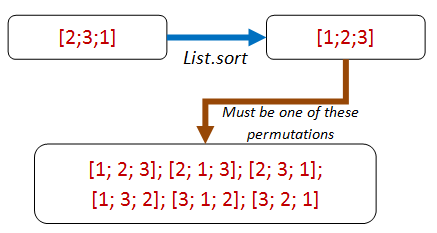
\includegraphics[width=1\textwidth]{images/property_list_sort_permutation.png}
            \caption{Strategia - niezmienność}
            \label{fig:invariant_strategy_example}
        \end{figure}    
    \end{columns}
\end{frame}


\begin{frame}{Strategie - Z czasem rzeczy\\przestają się zmieniać}
    \begin{columns}[t]
        \column{.5\textwidth}
            Inną właściwością funkcji może być niezmienność wyniku funkcji po ponownym jej zaaplikowaniu. 
            Innymi słowy, wykonanie funkcji 2 razy daje taki sam efekt, jak jednokrotne jej zaaplikowanie.
            \onslide<2->{Przykładami takich operacji, dla których taki typ testu miałby zastosowanie to metoda \texttt{distinct} wykonana na danej liście, lub wykonanie \texttt{update} na danej bazie danych.}
        \column{.5\textwidth}
        \centering
        \begin{figure}
            \centering
            
\includegraphics[width=1\textwidth]{images/property_idempotence.png}
            \caption{Strategia - idempotentność}
            \label{fig:independance_strategy}
        \end{figure}    
    \end{columns}
\end{frame}

\begin{frame}[fragile]{Strategie - Dziel i rządź}
    \begin{columns}[t]
        \column{.5\textwidth}
            Istnieją sposoby na testowanie na podstawie właściwości jest wykorzystanie rekursywności struktur przekazywanych do funkcji, takich jak \texttt{listy}, \texttt{drzewa}. 
            \onslide<2->{
                Przykładem może być sprawdzenie za pomocą tej metody funkcji sort.
            }
        \column{.5\textwidth}
            \centering
            \begin{figure}
                \centering
                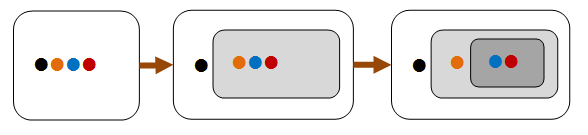
\includegraphics[width=1\textwidth]{images/property_induction.png}
                \caption{Strategia - rekursywna}
                \label{fig:recursive_strategy}
            \end{figure}    
    \end{columns}
\end{frame}

\begin{frame}[fragile]{Strategie - Dziel i rządź}
    \begin{lstlisting}[language=FSharp, xleftmargin=-10pt,xrightmargin=-10pt,numbers=none, basicstyle=\ttfamily\small]
    let rec firstLessThanSecond_andTailIsSorted sortFn 
    (aList:int list) =
        let sortedList = aList |> sortFn
        match sortedList with
        | [] -> true
        | [first] -> true
        | [first;second] -> first <= second
        | first::second::rest->
            first <= second &&
            let tail = second::rest
            // check that tail is sorted
            firstLessThanSecond_andTailIsSorted sortFn tail
    \end{lstlisting}
\end{frame}

\begin{frame}{Strategie - Łatwiej zweryfikować niż\\zaimplementować}
    \begin{columns}[t]
        \column{.5\textwidth}
            Niekiedy testowana funkcja jest skomplikowana, ale jej rezultat da się łatwo sprawdzić. Przykładem może być funkcja wyszukująca wyjście z labiryntu, gdzie sam algorytm wyszukiwania odpowiedniej ścieżki jest skomplikowany, 
            natomiast samo sprawdzenie, czy ścieżka dobrze prowadzi do wyjścia można w łatwy sposób zweryfikować.
        \column{.5\textwidth}
        \centering
        \begin{figure}
            \centering
            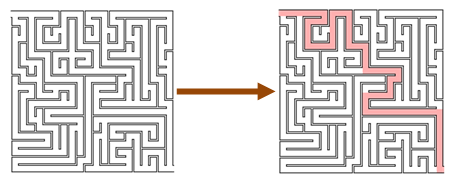
\includegraphics[width=1\textwidth]{images/property_easy_verification.png}
            \caption{Strategia - łatwe sprawdzenie}
            \label{fig:easy_verification_strategy}
        \end{figure}    
    \end{columns}
\end{frame}

\begin{frame}{Strategie - Łatwiej zweryfikować niż\\zaimplementować}
    \begin{columns}[t]
        \column{.5\textwidth}
            Niekiedy testowana funkcja jest skomplikowana, ale jej rezultat da się łatwo sprawdzić. Przykładem może być funkcja wyszukująca wyjście z labiryntu, gdzie sam algorytm wyszukiwania odpowiedniej ścieżki jest skomplikowany, 
            natomiast samo sprawdzenie, czy ścieżka dobrze prowadzi do wyjścia można w łatwy sposób zweryfikować.
        \column{.5\textwidth}
        \centering
        \begin{figure}
            \centering
            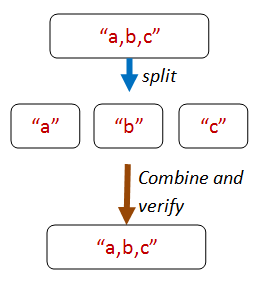
\includegraphics[width=0.7\textwidth]{images/property_string_split.png}
            \caption{Strategia - łatwe sprawdzenie}
            \label{fig:easy_verification_strategy_example}
        \end{figure}    
    \end{columns}
\end{frame}

\begin{frame}[fragile]{Strategie - Łatwiej zweryfikować niż\\zaimplementować}
    \begin{lstlisting}[language=FSharp, xleftmargin=-10pt,xrightmargin=-10pt,numbers=none, basicstyle=\ttfamily\small]
    let concatElementsOfSplitString_eq_originalString (strings:string list) =
        // make a string
        let inputString = strings |> String.concat ","
      
        // use the 'split' function on the inputString
        let tokens = stringSplit inputString
      
        // build a string from the tokens
        let recombinedString = tokens |> String.concat ","
      
        // compare the result with the original
        inputString = recombinedString
    \end{lstlisting}
\end{frame}

\begin{frame}{Strategie - Testowanie z wyrocznią}
    \begin{columns}[t]
        \column{.65\textwidth}
            Zdaża się, że funkcjonalność została już napisana i trzeba ją zrefactorować, przepisać, napisać od nowa. Warto wtedy wykorzystać wartości zwracane przez oryginalnie zaimplementowany algorytm jako pewną wartość wyniku, pewnego rodzaju wyrocznię, uznając go jako prawdę.
            \onslide<2->{W taki sposób można sprawdzić, czy nowa funkcja w pewnym stopniu pokrywa się ze starą funkcją. Czasami też istnieje wiele algorytmów doprowadzających do tego samego wyniku, mające różne złożoności, czy też działające równolegle.}
            \onslide<3->{Można wykożystać wtedy najprostrzy algorytm jako wyrocznię, ze względu na najmniejsze prawdopodobieństwo napisania takiego algorytmu z błędem. Następnie, przy wykorzystaniu wyroczni, stworzyć bardziej skomplikowany (często efektywniejszy) algorytm.}
        \column{.35\textwidth}
        \centering
        \onslide<1->{
        \begin{figure}
            \centering
            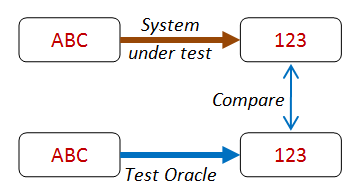
\includegraphics[width=1\textwidth]{images/property_test_oracle.png}
            \caption{Strategia - wyrocznia}
            \label{fig:oracle_strategy}
        \end{figure} 
        }   
    \end{columns}
\end{frame}
\begin{frame}{Cartpole}
    \fourImages{images/cartpole_w1.png}{images/cartpole_w2.png}{images/cartpole_w3.png}{images/cartpole_w4.png}    
\end{frame}
\begin{frame}{Cartpole}
    \begin{center}
        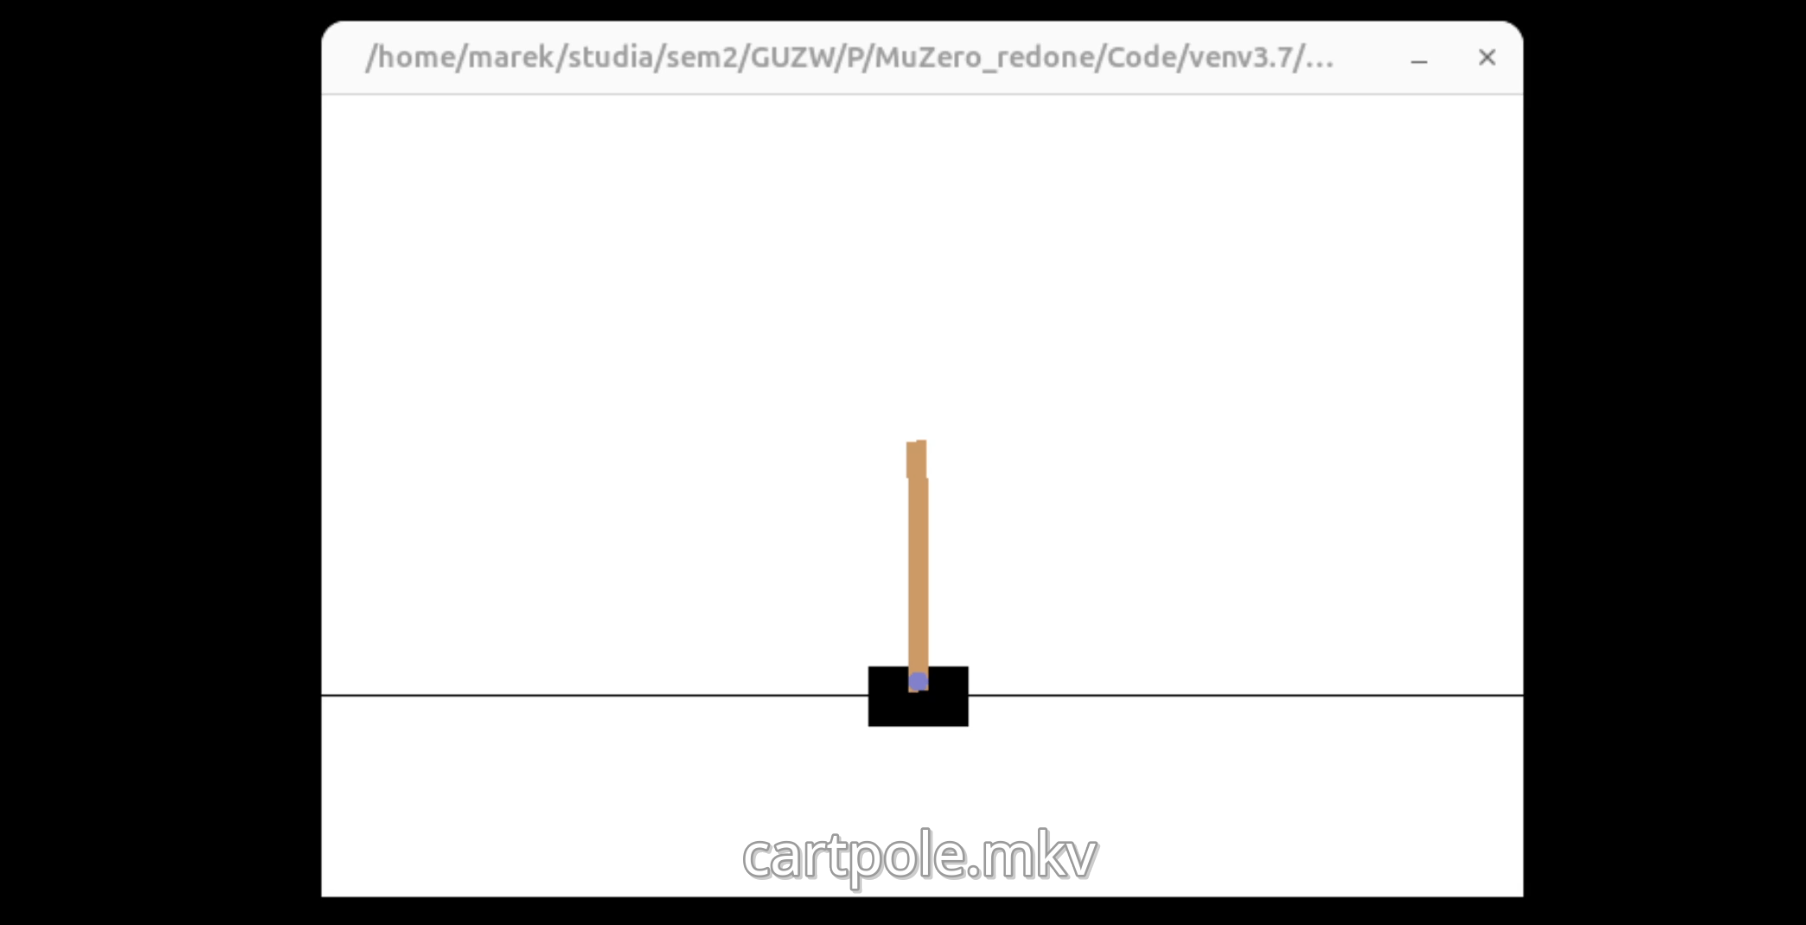
\includegraphics[height=.9\textheight,keepaspectratio]{images/cartpole_vid.png}
    \end{center}
\end{frame}
\begin{frame}{Gridworld}
    \fourImages{images/gridworld_w1.png}{images/gridworld_w2.png}{images/gridworld_w3.png}{images/gridworld_w4.png}    
\end{frame}
\begin{frame}{Gridworld}
    \begin{center}
        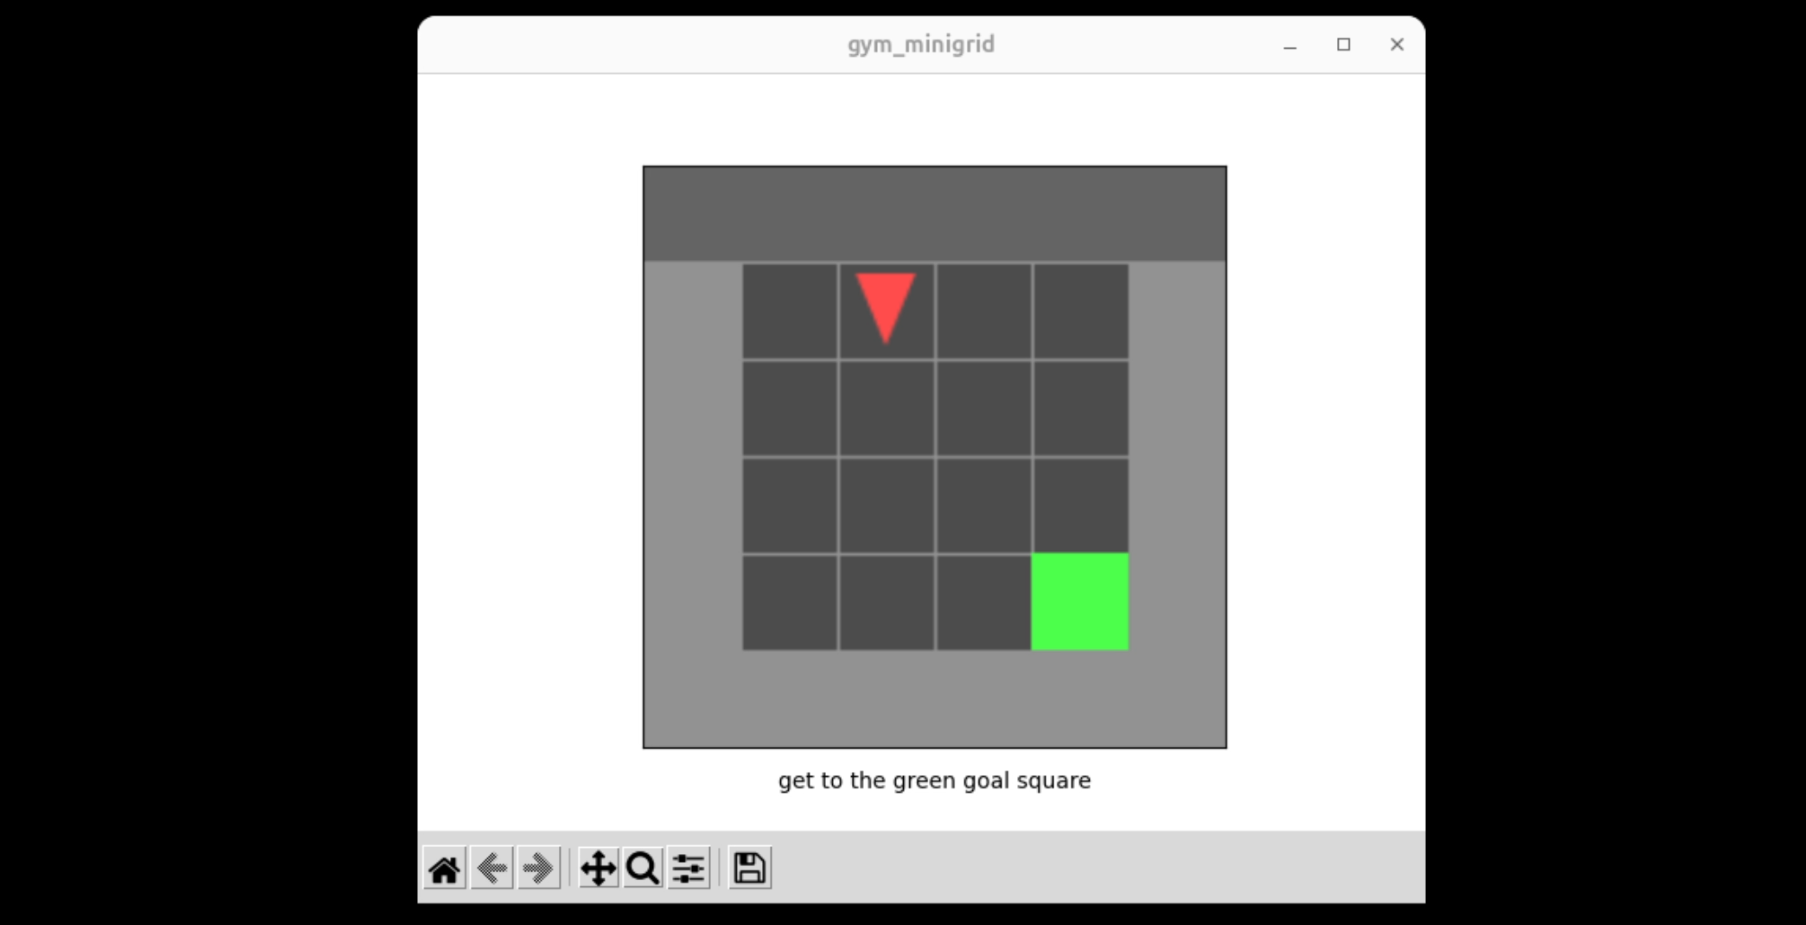
\includegraphics[height=.9\textheight,keepaspectratio]{images/gridworld_vid.png}
    \end{center}
\end{frame}
\begin{frame}{Breakout}
    \fourImages{images/breakout_w1.png}{images/breakout_w2.png}{images/breakout_w3.png}{images/breakout_w4.png}    
\end{frame}
\begin{frame}{Breakout}
    \begin{center}
        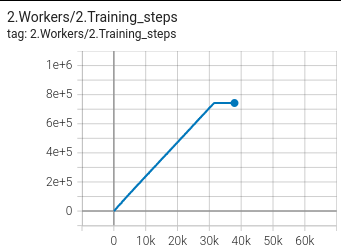
\includegraphics[height=.75\textheight,keepaspectratio]{images/breakout_problem.png}
    \end{center}
\end{frame}
\begin{frame}{Breakout 5M}
    \fourImages{images/breakout_v2_w1.png}{images/breakout_v2_w2.png}{images/breakout_v2_w3.png}{images/breakout_v2_w4.png}    
\end{frame}
\begin{frame}{Breakout GPU}
    \fourImages{images/breakout_gpu_w1.png}{images/breakout_gpu_w2.png}{images/breakout_gpu_w3.png}{images/breakout_gpu_w4.png}    
\end{frame}
\begin{frame}{Atlantis}
    \fourImages{images/atlantis_w1.png}{images/atlantis_w2.png}{images/atlantis_w3.png}{images/atlantis_w4.png}    
\end{frame}
\begin{frame}{Atlantis}
    \begin{center}
        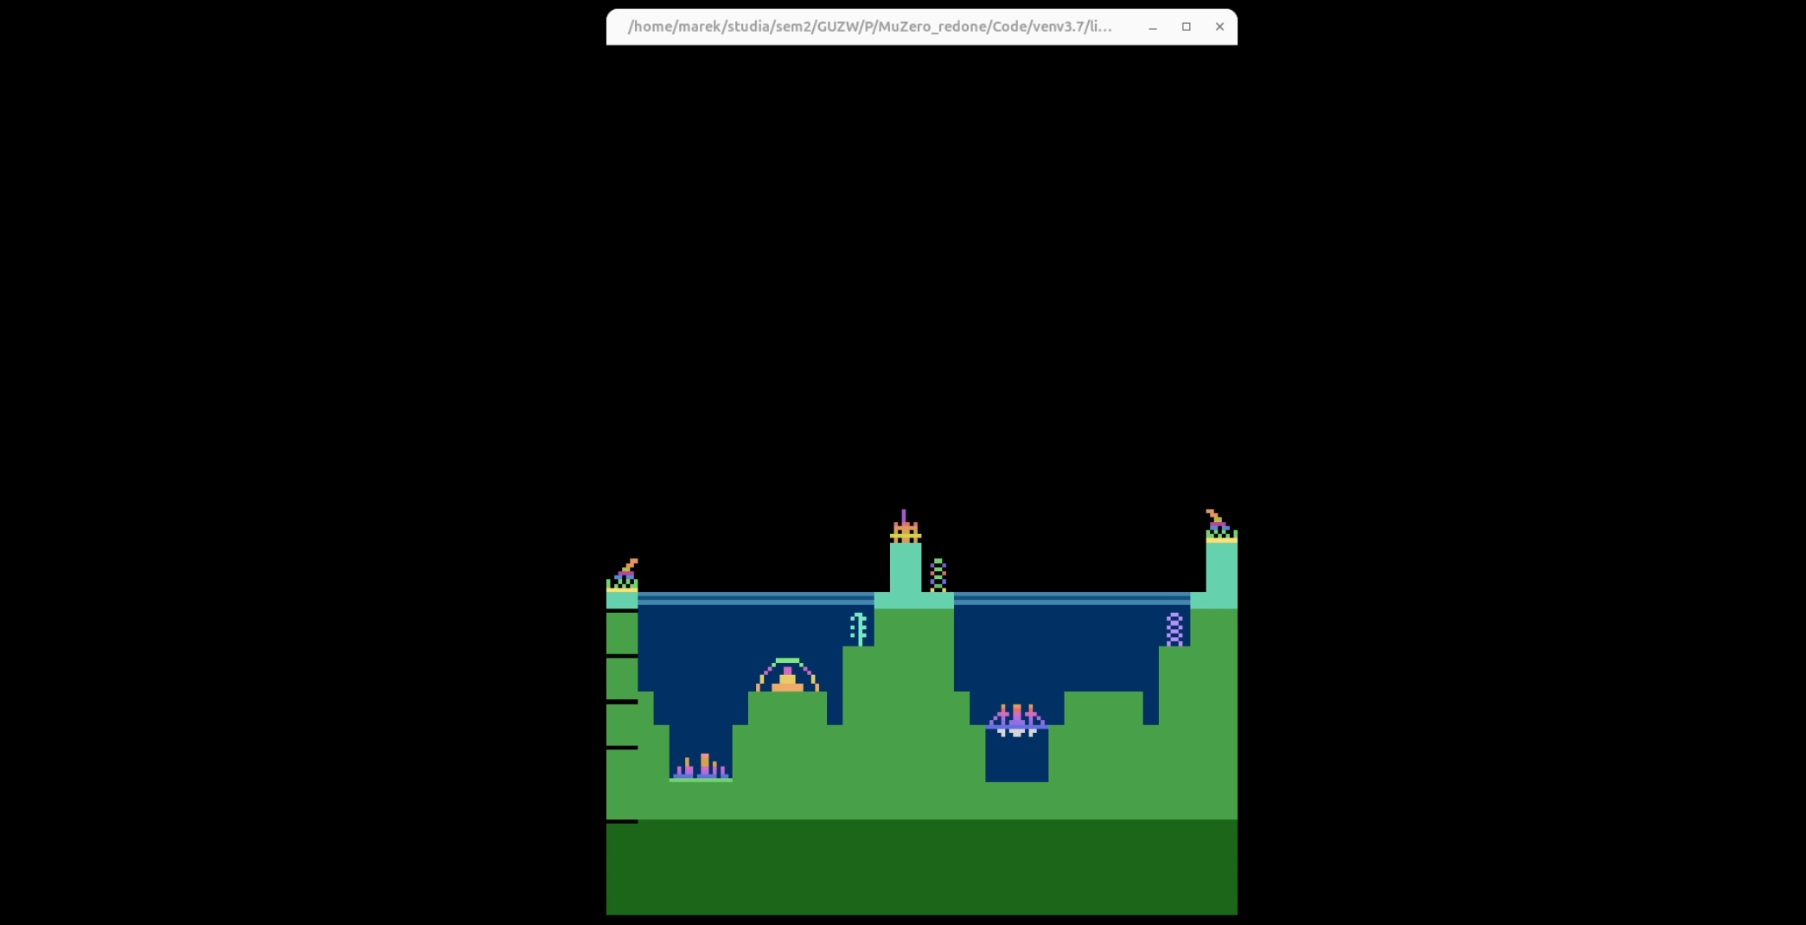
\includegraphics[height=.9\textheight,keepaspectratio]{images/atlantis_vid.png}
    \end{center}
\end{frame}
\begin{frame}{Bowling}
    \fourImages{images/bowling_w1.png}{images/bowling_w2.png}{images/bowling_w3.png}{images/bowling_w4.png}    
\end{frame}
\begin{frame}{Bowling}
    \begin{center}
        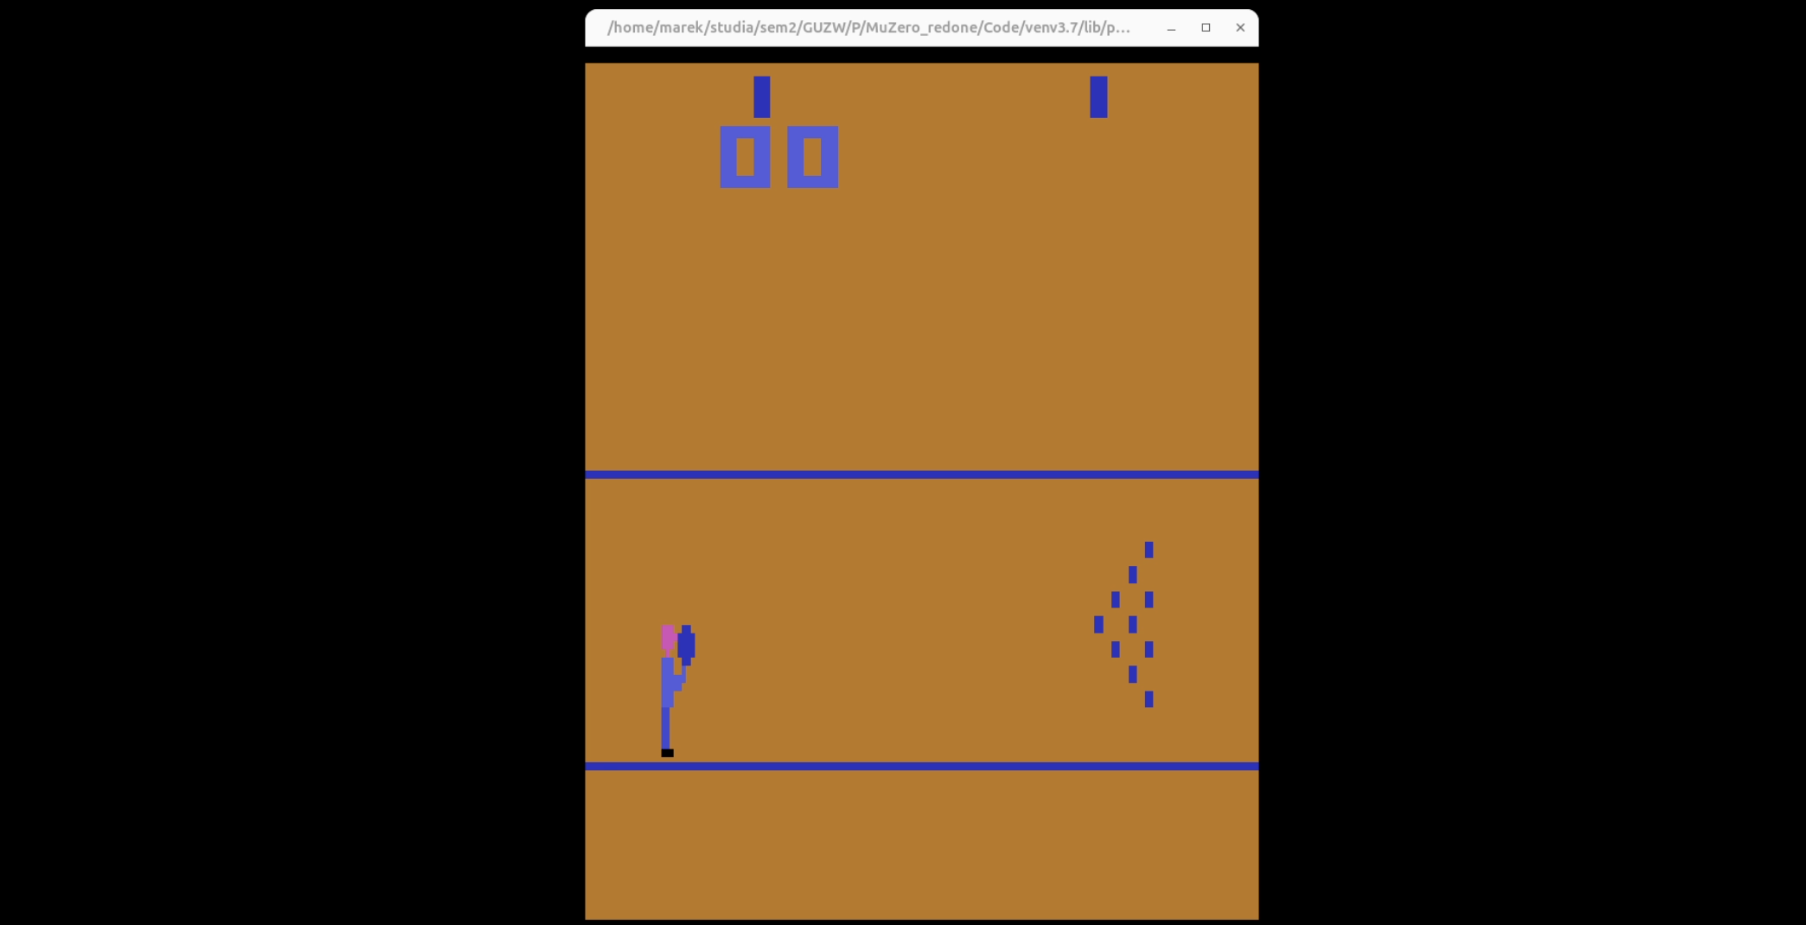
\includegraphics[height=.9\textheight,keepaspectratio]{images/bowling_vid.png}
    \end{center}
\end{frame}
\begin{frame}{Crazy climber}
    \fourImages{images/crazy_climber_w1.png}{images/crazy_climber_w2.png}{images/crazy_climber_w3.png}{images/crazy_climber_w4.png}    
\end{frame}
\begin{frame}{Crazy climber}
    \begin{center}
        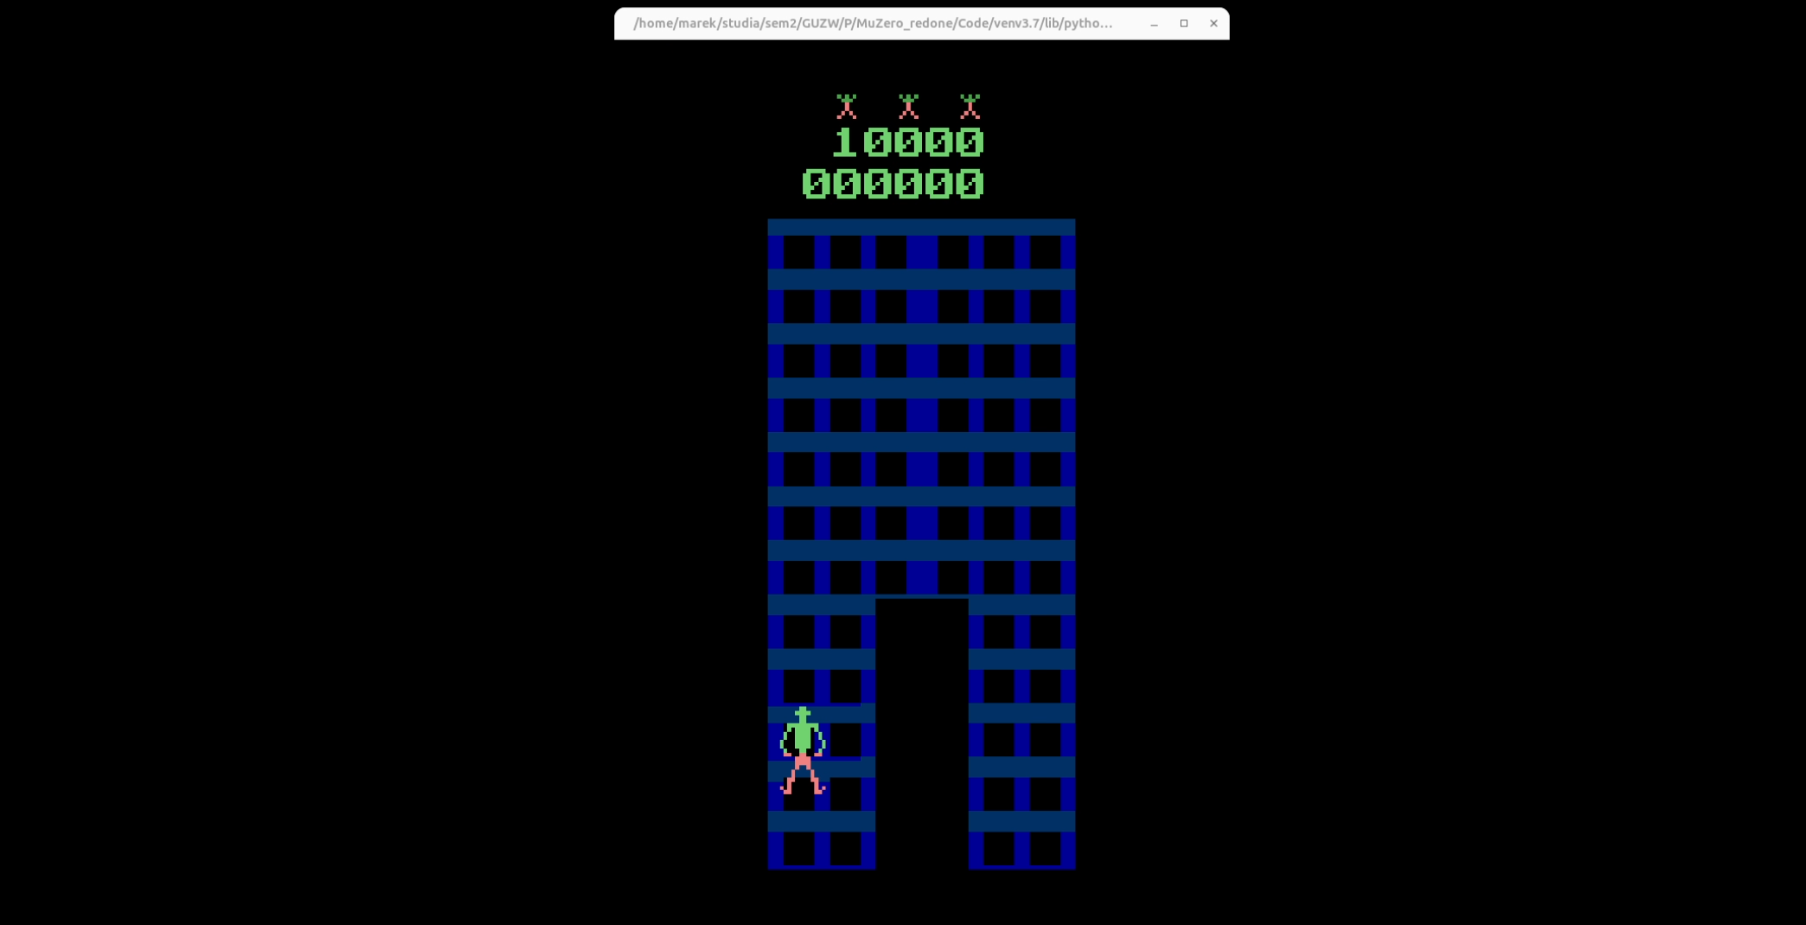
\includegraphics[height=.9\textheight,keepaspectratio]{images/crazy_climber_vid.png}
    \end{center}
\end{frame}
\begin{frame}{Pacman}
    \fourImages{images/pacman_w1.png}{images/pacman_w2.png}{images/pacman_w3.png}{images/pacman_w4.png}    
\end{frame}
\begin{frame}{Pacman}
    \begin{center}
        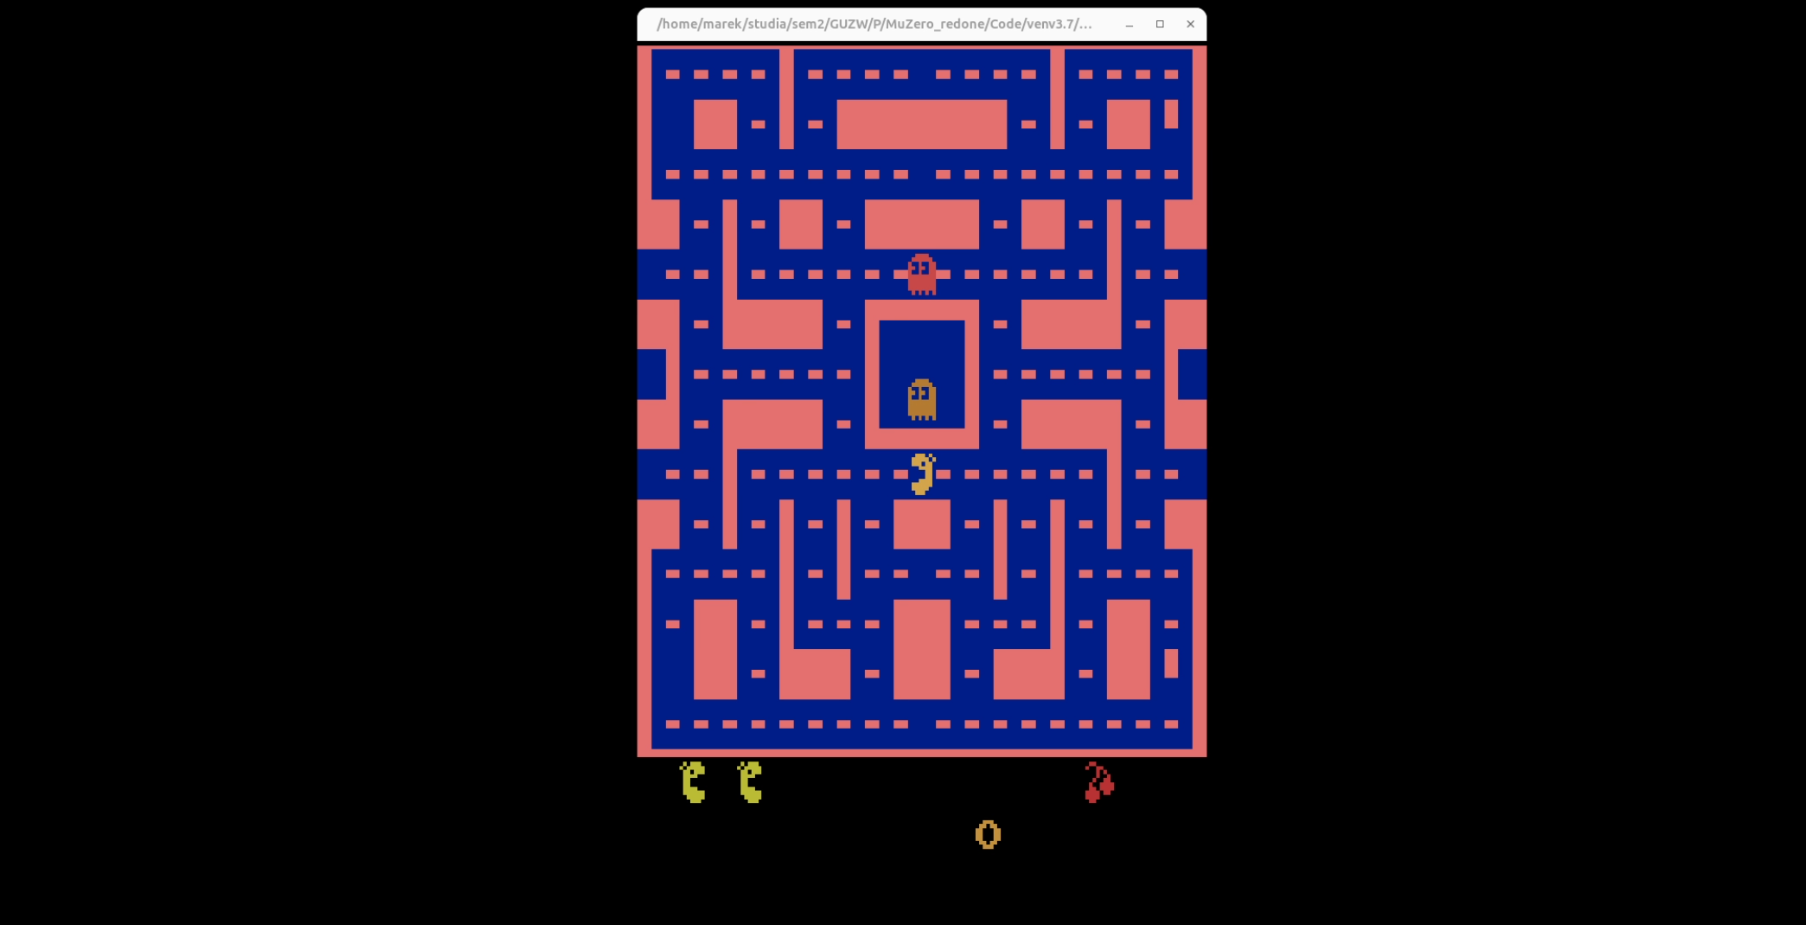
\includegraphics[height=.9\textheight,keepaspectratio]{images/pacman_vid.png}
    \end{center}
\end{frame}
\begin{frame}{Pong}
    \fourImages{images/pong_w1.png}{images/pong_w2.png}{images/pong_w3.png}{images/pong_w4.png}    
\end{frame}
\begin{frame}{Pong}
    \begin{center}
        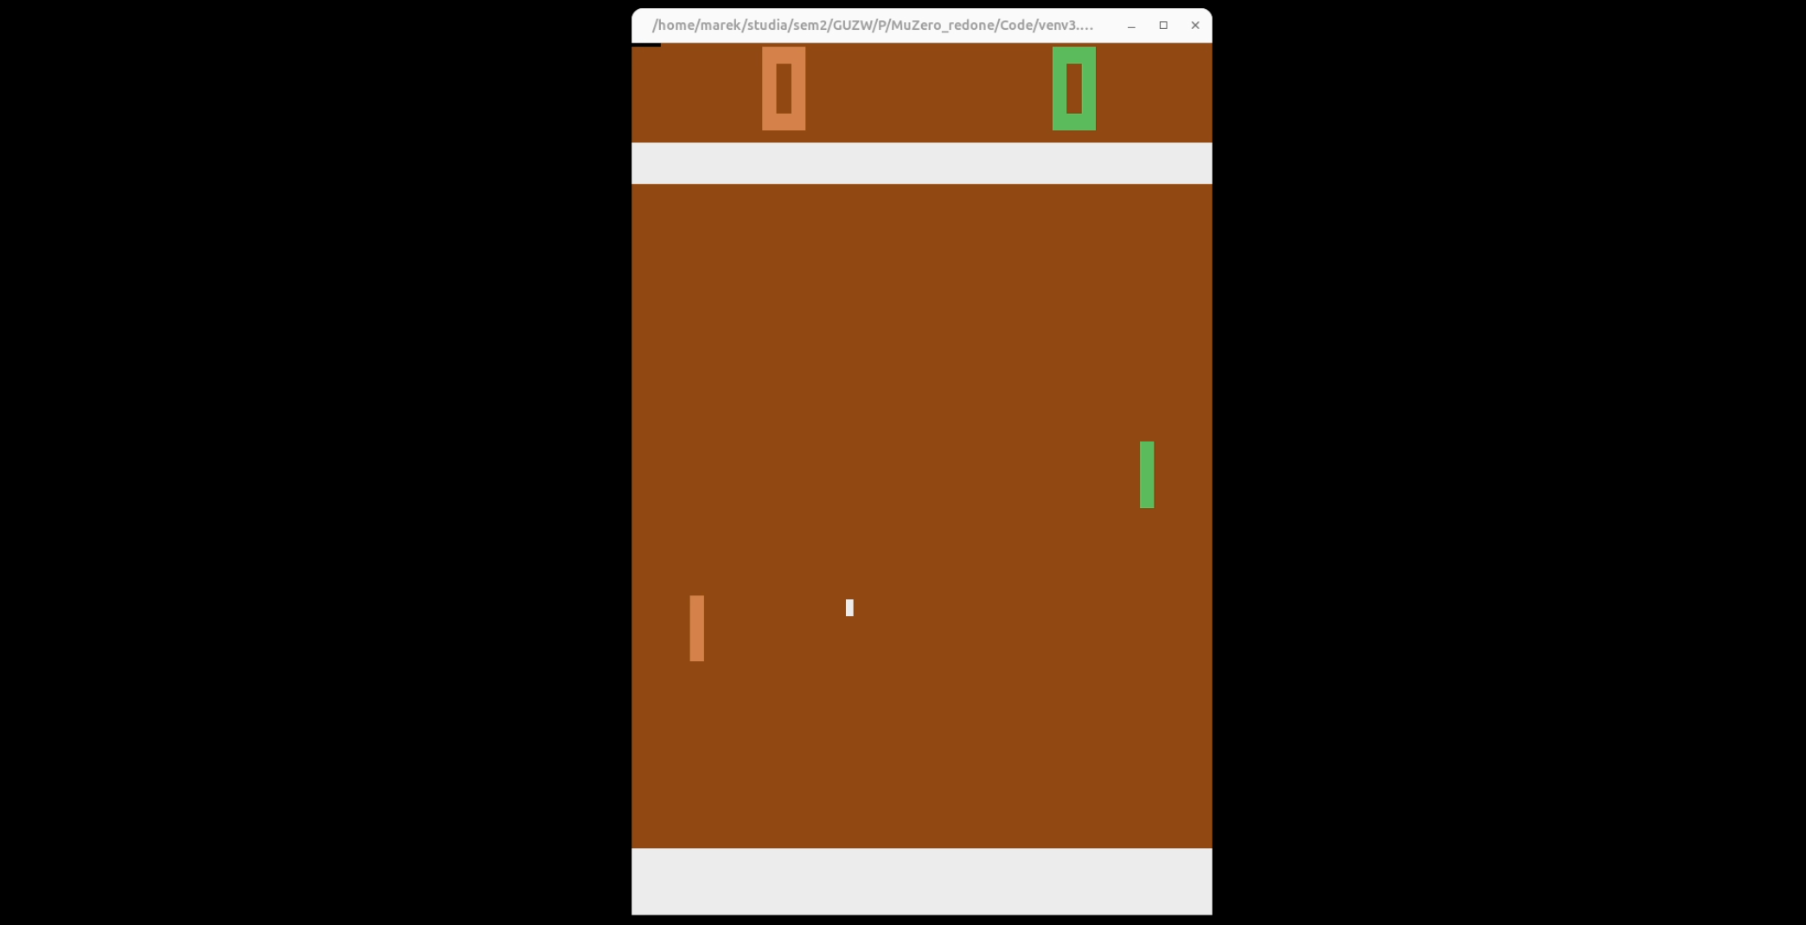
\includegraphics[height=.9\textheight,keepaspectratio]{images/pong_vid.png}
    \end{center}
\end{frame}
\begin{frame}{Doom}
    \fourImages{images/doom_w1.png}{images/doom_w2.png}{images/doom_w3.png}{images/doom_w4.png}    
\end{frame}
\begin{frame}{Doom}
    \begin{center}
        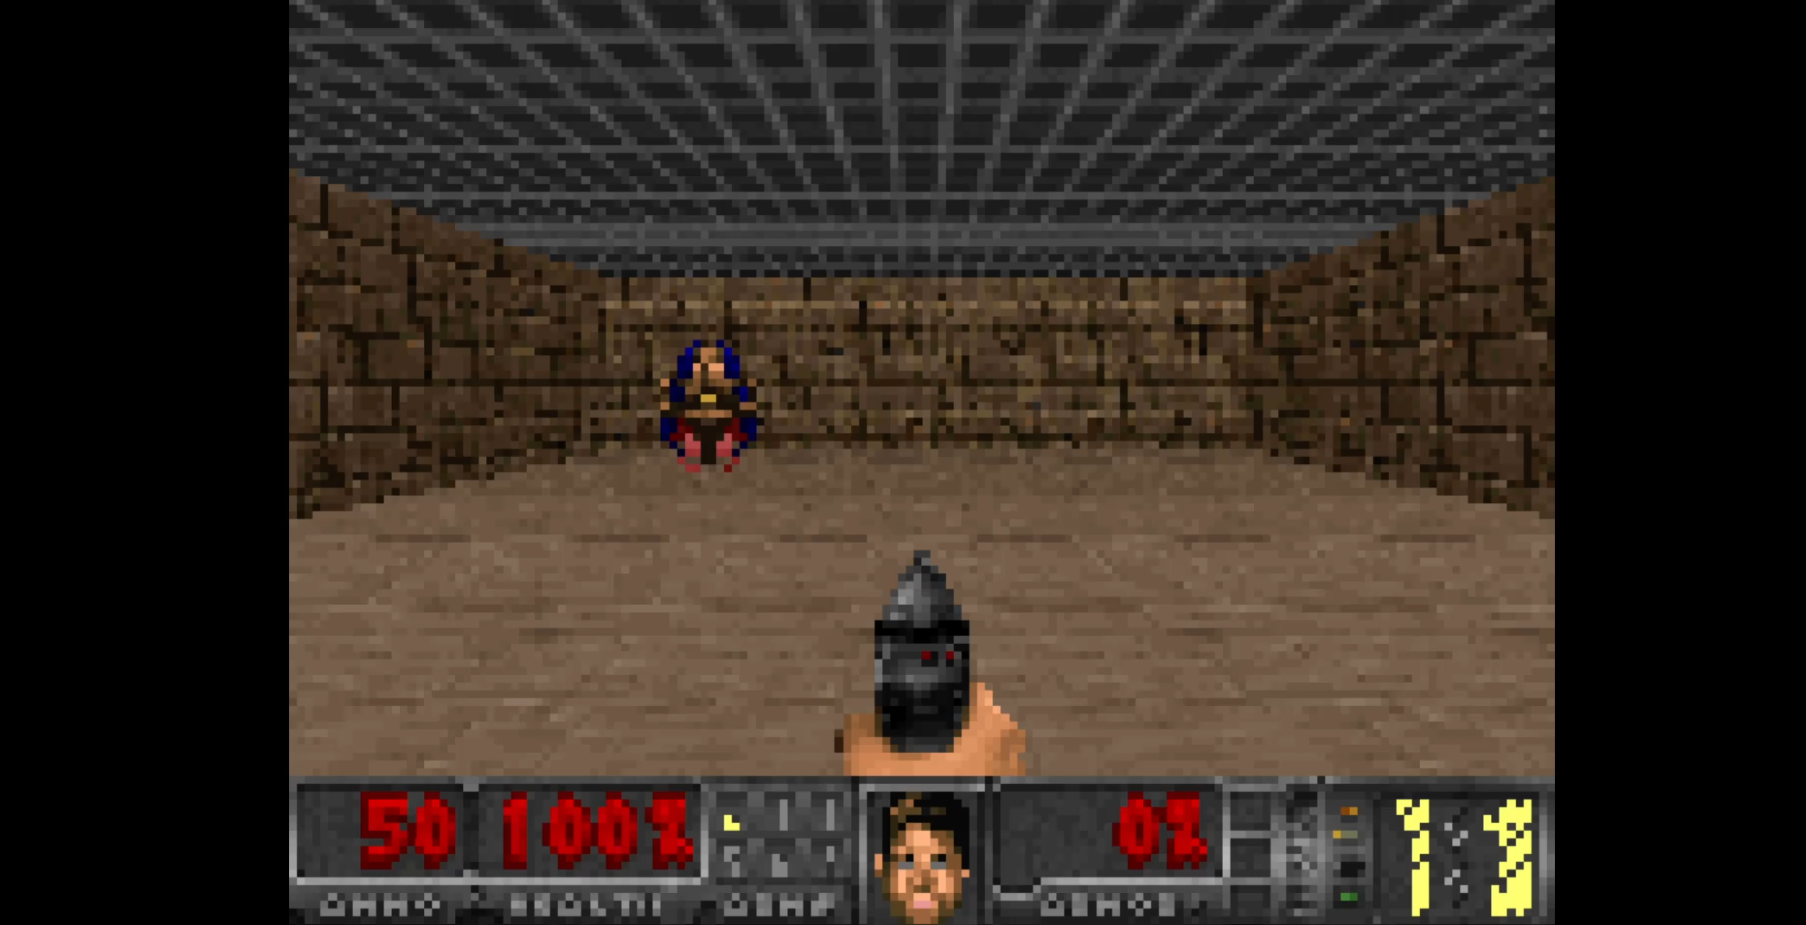
\includegraphics[height=.9\textheight,keepaspectratio]{images/doom_vid.png}
    \end{center}
\end{frame}
\begin{frame}{Podsumowanie}
    \begin{center}
        {\huge PODSUMOWANIE}
    \end{center}
\end{frame}
\begin{frame}{Pytania}
    \begin{center}
        {\huge Pytania?}
    \end{center}
\end{frame}

% \begin{frame}{Podziękowania}
%     Chcielibyśmy podziękować Panu dr. inż. Janowi Cychnerskiemu za stworzenie 
%     i udostępnienie stylu \href{https://github.com/jachoo/pg-beamer}{\emph{pg-beamer}}, 
%     co zostało wykorzystane do stworzenia tej prezentacji.\\
%     \url{https://github.com/jachoo/pg-beamer}
     
% \end{frame}

\begin{frame}{Koniec}
    \begin{center}
        {\huge Dziękujemy za uwagę!}
    \end{center}
\end{frame}

\pglastframe

\end{document}
